\section*{Integrated modeling framework}

The key idea of our approach is to constrain the parameters of a correlative meta-model using predictions made by one or several mechanistic sub-models from other spatial scales.
The role of the metamodel is to integrate data at the same ecological scale as predictions. 
As an example, the metamodel could take the form of a simple correlative \ac{SDM}.
Ideally, each sub-model incorporates different data types and hypotheses that specify underlying ecological mechanisms contributing to the model output.
The output of sub-models should provide additional predictions at a comparable ecological scale at which the metamodel operates, although it is not necessary for the sub-models to actually operate at the same scale.
For sub-models operating at a substantially different scale than the metamodel, scaling functions will be required; however, as we will show in the first example, these functions can be simple while still contributing useful information to the metamodel. 
All predictions may therefore be integrated in a single Bayesian framework when evaluating the parameters of the metamodel (see Box 1, Fig. \ref{fig:diagram}).
We present the complete framework in a hypothetical example where experimental results are  introduced as prior knowledge of the fundamental niche in a species distribution model (SDM).
A more formal presentation of the modeling framework appears in Box 1.
We follow with a second example where we apply our approach to integrate phenological information with occurrence data for a widespread North American tree.


\begin{figure}


%\documentclass{article}
%\usepackage{tikz}
%\usepackage{tikz-cd}
%\usepackage{amsmath}

%\usetikzlibrary{calc, shapes}
%\usetikzlibrary{shapes.geometric,shapes.arrows,decorations.pathmorphing}
%\usetikzlibrary{matrix,chains,scopes,positioning,arrows,fit}
%\begin{document}

%% --------------------------------------------------------------------------------------
%% ------part 1--------------------------------------------------------------------------
%% --------------------------------------------------------------------------------------

\begin{tikzpicture}
	
\matrix(m) [matrix of nodes, column sep=-0.5em,
	row sep=2em,
	minimum width=4em,
	minimum height=2em,
	column 1/.style={anchor=west, align=left, text width=10em},
	multi/.style={rectangle split,rectangle split parts=2}]
	{
	% zeroth line
	% blank space 
	&
	\textbf{Correlative Metamodel}
	&
	&
	\textbf{Mechanistic sub-model}
	\\
	% first line
	Data % m 1-1
	&
	$X_{M}, D_{M}$ % m 1-2
	&
	&
	$X_{S}, D_{S}$ % m 1-4
	\\
%second line
	|[multi]| Process % m 2-1 
	\nodepart{second}
	(prior and likelihood)
	&
	|[multi]|$p(\theta_{M})$ % m 2-2
	\nodepart{second}
	$p(X_{M} \mid \theta_{M}, D_{M})$
	&
	&
	|[multi]|$p(\theta_{S})$
	\nodepart{second}
	$p(X_{S} \mid \theta_{S}, D_{S})$
	\\

%third line
	
	Posterior
	&
	$p(\theta_{M} \mid X_{M}, D_{M})$
	&
	&
	$p(\theta_{S} \mid X_{S}, D_{S})$
	\\

%fourth line
	Prediction
	&
	$\psi_N = f(\theta_M, D_M)$
	&
	&
	$\psi_S = g(\theta_S, X_S, D_S)$
	\\

%fifth line
	Data
	&
	&
	&
	$\psi_S$
	\\
%sixth line
	|[multi]| Process
	\nodepart{second}
	(integrated likelihood)
	&
	$p(\theta_M \mid X_M, D_M)$
	&
	&
	$p(\psi_S \mid \theta_M)$
	\\


%seventh line
	Integrated posterior
	&
	&
	$p(\theta_M \mid \psi_S, X_M, D_M)$
	&
	\\

%eighth line
	Integrated prediction
	&
	&
	$\psi_I = f(\theta_M, D_M)$
	&
	\\
}; %end matrix

% The names of the nodes are automatically generated in the previous matrix. Since the
% matrix was named ``m'', all nodes have the name m-row-column

% metamodel
\draw [->] (m-2-2.south) -- (m-3-2.north);
\draw [->] (m-3-2.south) -- (m-4-2.north);
\draw [->] (m-4-2.south) -- (m-5-2.north);

%%mechanistic model
\draw [->] (m-2-4.south) -- (m-3-4.north);
\draw [->] (m-3-4.south) -- (m-4-4.north);
\draw [->] (m-4-4.south) -- (m-5-4.north);

%%separation line
\draw [line cap=rect, transform canvas={yshift=-1em}] (m-5-1.south west) -- (m-5-4.south east);
%(\linewidth-\pgflinewidth,0); 

\tikzstyle{opt}=[gray,dashed,rounded corners];
\draw [->,style=opt] (m-4-2.west) to[bend right=50] (m-7-2.west);
\draw [->,style=opt] (m-5-4.south) to (m-6-4.north);

%%integrated model
\draw [->] (m-7-2.south) -- (m-8-3.north west);
\draw [->] (m-6-4.south) -- (m-7-4.north);
\draw [->] (m-7-4.south) -- (m-8-3.north east);
\draw [->] (m-8-3.south) -- (m-9-3.north);


\end{tikzpicture}


\caption{The parameters of a correlative metamodel model (left column) are conditioned on the predictions of a mechanistic sub-model (right column).
The metamodel ($\theta_M$) operates at a single ecological scale and uses occurrence data (\(X_M\)) and explanatory variables ($D_M$) to produce a naive (i.e., not conditioned on sub-models) prediction $\psi_N$.
The mechanistic sub-model \(\theta_S\) includes data about the response (\(X_S\)) of lower-level behaviours of the system to explanatory variables ($D_S$). 
The models are integrated by calibrating $\theta_M$ to data ($X_M, D_M$) as well as the output of the sub-model ($\psi_S$). 
This is possible because predictions from the sub-model ($\psi_S$) emerge at the scale of the metamodel via a scaling function \(g(\theta_S, D_S)\).
The final prediction can be obtained by applying the integrated model to the original explanatory variables (as shown) or, if projection is desired, on some new set of explanatory variables (e.g., future climate).
This prediction incorporates multiple sources of information coming from several calibration datasets (i.e., $X_M, D_M, X_S, $ and $D_S$) as well as from multiple types of models (i.e., $\theta_M$ and $\theta_S$).
}
\label{fig:diagram}
\end{figure}


%---------------------------------------------
\subsection*{Example 1: Adding experimental evidence for the fundamental niche to a species distribution model} 

In this hypothetical example, we build a metamodel relating the distribution (i.e. occurrence probability) of an annual plant to coarse-scale climate with complementary information originating from a fine-scale experiment manipulating the precipitation regime.
The metamodel attempts to capture the realized distribution of a species; as a correlative model, it implicitly captures the major physiological constraints and ecological processes constraining the distribution of the target species. 
However, for the purposes of forecasting, we would like to disentangle the fundamental response of a species to environmental variation from other processes in order to map the climatic envelope of where a species may be found in a natural setting. 
Prior information of the physiological constraints affecting species distribution is sometimes available, but usually too incomplete to perform a reasonable comparison with the realized distribution.
For instance, as in this example, a species distribution might be constrained by both temperature and precipitation, but experiments were conducted only over a precipitation gradient at one temperature. 
We apply our framework here to such heterogeneous sources of information to reduce the bias in parameter estimation and more adequately represent uncertainty. 
Here, we focus only on the specification of the modeling framework; complete procedural details and code for generating the data sets and executing the model are provided as supplemental information.

We consider data collected from a species' historical distribution, where the goal is to predict the distribution following a substantial reduction in precipitation. 
We will consider \(X_M\) (see Box 1, Fig. \ref{fig:diagram}) to be a vector of $n$ observations that takes the value of one to indicate presence and zero for absence:
\begin{equation}
X_M = \{x_{M,1}, x_{M,2}, \ldots, x_{M,n}\}
\end{equation}
We further assume the data are relatively high-quality, providing coverage over a wide region and covering various climatic conditions (Fig. \ref{fig:ex1_sampling}a). 
The model is evaluated by relating these observations to environmental data \((D_M)\), which for the sake of the example consists of mean annual temperature $T_M$ and annual precipitation $P_M$. 
For simplicity, we use a simple logistic model for the metamodel \((\theta_M)\) with a second order effect of temperature and precipitation. 
This naive model (i.e., the metamodel with no constraints from sub-models) predicts  occurrence probability (\(\psi_N\)) as a function of the environment:
%-----
\begin{equation}
\begin{aligned}
	\psi_N &= f\left(\theta_M, D_M \right) \\
	&= p \left (X_M = 1 \mid \theta_M, T_M, P_M \right) \\
	&=\text{logit}^{-1}\left( \mathbf{\Theta_M} \mathbf{D_M} \right)
\end{aligned}
\end{equation}
%-----
where \(\mathbf{\Theta_M}\) is the parameter vector of the model \(\theta_M\), \(\mathbf{D_M} \) is the covariate matrix (i.e., \(T_M, P_M\), with the first column taken to be unity to allow an intercept to be fit), and \(\text{logit}^{-1}\) is the inverse of the logit function.
We can fit this model in a Bayesian framework to allow for easy integration of models (as we will show later).
In this context, the goal of modeling is to estimate the probability distribution of \(\theta_M\), the model parameters, given the observed data \((X_M, T_M, P_M)\), which is given by the proportional form of Bayes's Theorem \citep[for readers unfamiliar with general concepts in Bayesian inference, concise introductions can be found in ][]{McCarthy2007, Link2010}:
%-----
\begin{equation}
\label{eq:ex1_bayes}
	p\left (\theta_M \mid X_M,T_M,P_M \right ) \propto 
	p \left(X_M \mid \theta_M, T_M, P_M \right)
	p \left(\theta_M \right)
\end{equation}
%-----
where \(p\left(X_M \mid \theta_M, T_M, P_M \right)\) is often referred to as the \emph{likelihood} of the data (\(X_M\)) given the model (\(\theta_M\)), \(p\left(\theta_M \right)\) is often referred to as the \emph{prior distribution} of \(\theta_M\), and the goal of modeling is to estimate \(p\left (\theta_M \mid X_M,T_M,P_M \right )\), the \emph{posterior distribution} of \(\theta_M\), which gives the probability that \(\theta_M\) takes particular values, given the observed data.

%==================
% FIGURE

\begin{figure}[tb]
	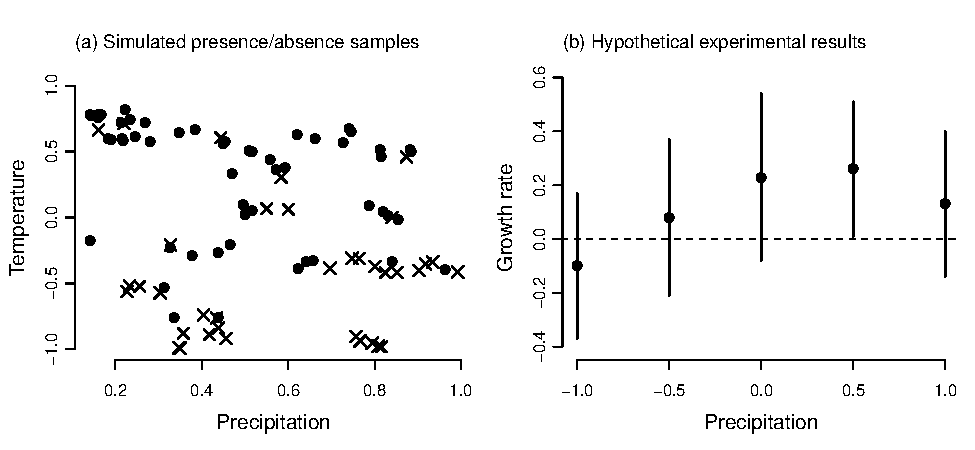
\includegraphics{ex1_sampling.pdf}
	\caption{Two simulated data sets used to illustrate the model integration framework.
	(a) Presences (circles) or absences (x's) of the species in ecological space, where precipitation ranges from 0--1.
	(b) Growth rate ($r$) as a function of manipulations to the precipitation regime (whiskers show $\pm$ 1 SE), with a larger range for precipitation (i.e., \(-\)1--1).
	The dashed line shows the threshold above which the species net growth rate is positive (implying presence).
	Axis scales for temperature and precipitation are arbitrary, but note the different scales on the horizontal axes.}
	\label{fig:ex1_sampling}
\end{figure}

% ERUGIF
%==================

Thus far, we have considered only a single source of information to fit this model, and therefore the prior distribution \(p\left(\theta_M \right)\) from Eq. \ref{eq:ex1_bayes} is uninformative.
As a secondary source of information, we will consider an experiment relating the population growth rate of the plant to manipulations to the precipitation regime, with results (but no raw data) available from the literature (Fig. \ref{fig:ex1_sampling}b). 
Furthermore, no information is available regarding the temperature regime for the experiment.
Transplant experiments that evaluate performance beyond the range of a species are common, and represent a plausible scenario for model integration \citep{Hargreaves2014}.
According to niche theory \citep{Holt2009}, the fundamental niche corresponds to the set of environmental conditions where the per capita intrinsic growth rate $r$ is positive.
This concept gives us a reasonable model to fit the scaling function $g$ for our sub-model (Fig. \ref{fig:diagram}).
If we hypothesize that the errors from Figure \ref{fig:ex1_sampling}b \( \left(\sigma_{S} \right) \) are normally distributed, then for observation $i$, we can interpret the probability of presence \( \left(\psi_{S,i}\right)\) as the probability that the observed growth rate \(X_{S,i}\) is positive:
\begin{equation}
	\psi_{S,i} = \int_0^\infty N \left(X_{S,i}, \sigma_{S,i} \right)
\end{equation}
where \(N\) is the Normal density function.
We can then estimate the posterior distribution for the sub-model by fitting the relationship between \(\psi_S\) and precipitation \( \left( P_S \right) \) using Bayesian beta regression \citep{Ferrari2004}:
%-----
\begin{equation}
\label{eq:ex1_thetas}
	p\left (\theta_S \mid \psi_S,P_S \right ) \propto 
	p \left(\psi_S \mid \theta_S, P_S \right)
	p \left(\theta_S \right) \\
\end{equation}
%-----

Although the two data sets were collected at considerably different scales, we now have sub-model predictions arising from a fine-scale experiment that are relevant at the scale of the metamodel (i.e., the probability of presence at a given precipitation). 
This scaling is quite simplistic, and would never be used to predict a species' range using this mechanistic sub-model in isolation.
Despite the strong theoretical foundation (i.e., niche theory) linking the observations to presence-absence at large scales, the upscaled sub-model (i.e., the transformation of \(X_S\) and \(\sigma_S\) to \(\psi_S\)) is built on the strong hypothesis that the species will be present when $r>0$, neglecting other population dynamics constraints such as Allee effects and metapopulation dynamics. 
The fundamental niche is also incomplete, as we lack environmental variables such as temperature, as well as all other ecological processes responsible for the realized distribution.
As such, it would be unwise to expect predictions from this model alone to resemble the actual distribution of the species; as a mechanistic model, it is simply too incomplete to predict distribution.
As we will show, however, the information from this sub-model, when applied as a constraint on the metamodel, can result in improved predictions that incorporate the information within each model.

We accomplish model integration by treating the posterior of \(\theta_S\) as prior information about some of the parameters of \(\theta_M\) (i.e., parameters related to precipitation), expanding Equation \ref{eq:ex1_bayes} to incorporate the new information from the sub-model:
%-----
\begin{equation}
	\label{eq:ex1_integrated}
	\overbrace{p(\theta_M \mid X_M, T_M, P_M, \theta_S, \psi_S, P_S)}^\text{integrated posterior}
	\propto
	\overbrace{p\left (\psi_S \mid \theta_S,P_S \right )}^{\substack{\text{new information} \\ \text{from sub-model}}}
	\overbrace{p \left(X_M \mid \theta_M, T_M, P_M \right) P \left(\theta_M \right)}^{\substack{\text{naive metamodel} \\ \text{posterior}}}
	\overbrace{p \left(\theta_S \right)}^{\substack{\text{prior for} \\ \text{sub-model}}}	
\end{equation}
%-----
As before, the metamodel \(\theta_M\) can be used to predict the species distribution \((\psi_I)\).
However, these predictions will not reflect only the presence-absence samples in \(X_M\), but will also reflect the information from \(\theta_S\), including all of the data sources used to produce this sub-model.
In other words, with this evaluation, the set of parameters $\theta_M$ is most likely when it agrees with both the original data and predictions from the sub-model. 
Note that in this particular example, because the sub-model is only contingent on precipitation, there is no integration on temperature. 
Finally, we note the presence of marginal distributions for both models (i.e., \(p(\theta_M)\) and \(p(\theta_S)\)).
These can be informative (e.g., incorporating further prior information or the predictions of additional sub-models), semi-informative (e.g., to provide greater weight to more informative models), or uninformative.
For purposes of this example, we used these terms to reduce the precision of the second model to reflect the uncertainty of the modeling process (due to the lack of additional mechanisms in the second model, as mentioned above).

We performed this procedure with our hypothetical data sets.
When comparing the three models (naive metamodel, mechanistic sub-model, and integrated metamodel), we observed extreme uncertainty in the first model when projecting beyond the range of the original data.
Unsurprisingly given the quality of the data, the sub-model was highly precise, providing a fairly strong constraint when producing the integrated model.
The result was an integrated prediction that reflected the shapes of both models and showed considerably reduced uncertainty (Fig. \ref{fig:ex1_precip}).
At the scale of the metamodel, considering both temperature and precipitation, we observed similar results, with reduced uncertainty in the predictions over the domain not covered by the presence-absence data (Fig. \ref{fig:ex1_map}).


%==================
% FIGURE

\begin{figure}[tb]
	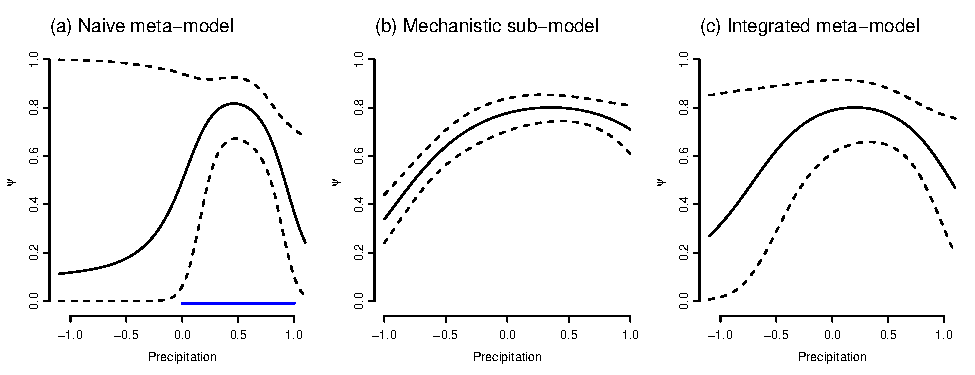
\includegraphics{ex1_precip.pdf}
	\caption{Results of integration showing the probability of presence (\(\psi\)) when considering only precipitation.
	(a) Naive model, using only presence-absence data. Uncertainty increases dramatically when attempting to project beyond the scope of the source data (represented by the horizontal line above the bottom axis).
	(b) Mechanistic model, using observations of an experiment to infer probability of presence. Predictions are highly precise due to high quality source data, but are likely to be overly optimistic given the simplicity in assuming only precipitation determines probability of presence (see text).
	(c) Integrated model, showing predictions that are intermediate between the two sub-models and uncertainty that is reduced compared to (a).
	Uncertainty is represented as dashed lines, showing the limits of 90\% Bayesian credible intervals.}
	\label{fig:ex1_precip}
\end{figure}
% ERUGIF
%==================


%==================
% FIGURE

\begin{figure}[tb]
	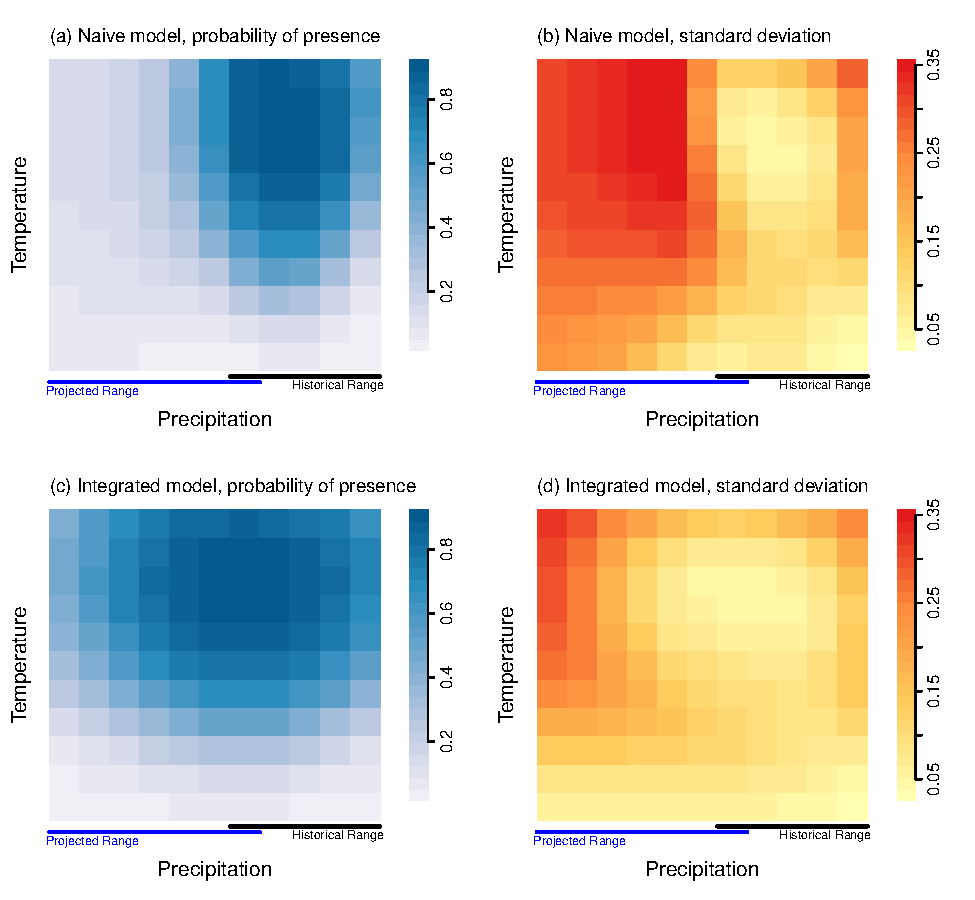
\includegraphics[width=5.25in]{ex1_map.pdf}
	\caption{Maps showing the predicted probability of presence (\(\psi\); (a) and (c)) and the standard deviation of \(\psi\) ((b) and (d)) for the naive and integrated models.
	Historical (e.g., where presence-absence samples were available) and predicted future precipitation regimes are shown below the horizontal axes.
	Uncertainty in the naive model was extreme when predicting beyond the historical precipitation regime.
	Uncertainty in the integrated model was considerably reduced, reflecting the additional information provided by the mechanistic model.}
	\label{fig:ex1_map}
\end{figure}
%
% ERUGIF
%==================

Once the technical challenges of evaluating the parameters are overcome, the integration has several advantages over the both the naive parameterization of the metamodel and the mechanistic sub-model. 
In the situation where both models strongly agree on the relationship between water availability and occurrence probability, then we should expect significantly reduced uncertainty in that domain (Figs. \ref{fig:ex1_precip}, \ref{fig:ex1_map}).
Because the metamodel includes both temperature and precipitation, any reduction in the uncertainty with respect to precipitation might also influence the evaluation of the relationship with temperature (reducing bias in the case where there is a correlation between T and P in the data). 
However, uncertainty could increase in the case of model disagreement.
For instance, the relationship between precipitation and presence in the naive metamodel could be caused by a spurious relationship (e.g. spatial autocorrelation caused by historical contingencies), leading to a false confidence in the species distribution over precipitation gradients. 
The information from the sub-model will thus bring back the right amount of uncertainty in the relationship.
Moreover, convergence in model predictions in overlapping domains (e.g., near the peak in the probability of presence in Fig. \ref{fig:ex1_precip}) can aid in detecting crucial ecological processes.

\subsection*{Example 2: Constraining an SDM using phenological information}
For the second example, we consider the problem of predicting the future distribution of a species following climate change.
There is considerable interest in comparing correlative and mechanistic projections with respect to climate change \citep{Morin2009}, and correctly characterizing uncertainty is a critical aspect of this problem \citep{Cheaib2012}.
Despite being a relatively common application of \ac{SDM}s \citep{Guisan2005}, projecting models parameterized with modern climate data to future climate scenarios is problematic for a number of reasons previously discussed \citep{Araujo2006, Austin2011}.
We used our metamodeling framework to inform a climate-based SDM with information obtained from Phenofit, a mechanistic model that predicts a species' probability of presence as a function of the suitability of the environment given the species' phenology \citep{Chuine2001, Morin2009}.
We use data from \citet{Morin2009} for sugar maple (\emph{Acer saccharum}), an economically and ecologically important species occurring in eastern North America.
Here we describe briefly the dataset, methods, and the results of the analysis.
Complete details, including all data and scripts to reproduce the analysis, are included as supplemental information.

\defcitealias{IPCC2001}{IPCC, 2001} %% this is needed to make the organizational citation in the following paragraph work correctly
For the meta-model, we used a dataset of 1013 presence and 13863 absence records, at 0.5 degree resolution, sampled from North America.
We reserved one-third of the dataset for validation, and used the area under the receiver operating characters curve (AUC) for validation of contemporary predictions, and the coefficient of determination (\(R^2\)) as a measure of the fit between the future predictions of the metamodel and the Phenofit predictions.
We used a binomial GLM to relate the suitability for sugar maple to 6 climate variables, scaled to the same resolution (see supplemental information for a descriptions of the climate variables and of the model selection process).
We selected a GLM here for its simplicity and interpretability because our focus was on demonstrating the framework, but more complex methods (e.g., GAM) are compatible with the framework.
For projection, we used predictions for 2080 from the HadCM3 GCM \citep{Pope2000} driven by the A2 emission scenario (Nakicenovic2000), and used the parameters of the GLM to forecast suitability into the future (i.e., \(\psi_N\)).
Phenofit produces predictions at continental scales; thus the scaling function \(g\) was incorporated within Phenofit itself and we performed model integration directly on the outputs.
To perform the integration, we used \ac{MCMC} to condition the parameters of the metamodel  on two likelihood functions.
The first is the naive SDM, where the likelihood of a ``success'' in the presence/absence dataset was a Bernoulli density with the (logit-transformed) probability expressed as a linear function of the climate predictors.
For the sub-model, we considered that Phenofit, being a process-based model, may perform better when projecting into the future.
Thus, we used the predicted future probability of presence as the basis for generating simulated future presence-absence datasets.
This procedure inherently incorporates some uncertainty by randomly determining where the species is present (though uncertainty in the probabilities themselves could not be incorporated, as they were not available).
Thus, the sub-model likelihood is simply the probability of observing a simulated dataset (that is randomly drawn from the phenofit predictions \(X_s\)),  given the predictions of the metamodel, resulting in the following posterior probability for the integrated metamodel:
\begin{equation}
\label{eq:integrated2}
	p( \theta_M \mid X_M, D_M, X_S, \theta_S )
	\propto 
	p( X_S \mid \theta_M, \theta_S )
	p( Y_M \mid \theta_M, D_M ) 
	p( \theta_M )
	p( \theta_S )
\end{equation}
where \(\theta_M\) is the metamodel, 
\(X_M\) is the vector of contemporary presences and absences, 
\(D_M\) is the matrix of climate predictors,
\(X_S\) is the prediction from Phenofit,
and \(\theta_S\) is the model relating the Phenofit predictions to the metamodel.
Note that the simulated datasets do not appear in this formulation, as they are only generated during estimation as a function of \(X_s\), and vary randomly between individual steps of the Markov chain.
Furthermore, the integration is performed on the \emph{predictions} of the sub-model directly, rather than on compatible parameters as in Example 1. 
Thus, the metamodel must appear in the sub-model likelihood.

The naive model, despite being a relatively inflexible GLM based on 3 climatic variables
relatively simple (xx climate variables with xx total parameters), was highly fit to the data and consequently showed very high suitability scores near the core of the contemporary range with very little uncertainty (Fig \ref{fig:ex2}C, E).
Similar patterns were repeated for analogous climates under the future scenario (Fig \ref{fig:ex2}D, F).
However, standard errors were extreme for the range margins where suitability scores were intermediate.
In comparison, Phenofit suitability scores were more moderate, and Phenofit predicted less northward movement of sugar maple under the future scenario \citep[Fig. \ref{fig:ex2}A, B;][]{Morin2009}.
The integrated model demonstrated generally lower suitability scores throughout both the present and projected ranges, and thus represents lower confidence in the presence of sugar maple at any given location in its future projected range (Fig \ref{fig:ex2}G, H).
Standard errors at range margins were significantly lower (as these are regions where both the naive model and phenofit were in agreement about intermediate suitability scores), whereas standard errors were slightly higher at the core range (where Phenofit predicted lower suitability than the naive model) (Fig \ref{fig:ex2}I, J).

%==================
% FIGURE

\begin{figure}[tb]
	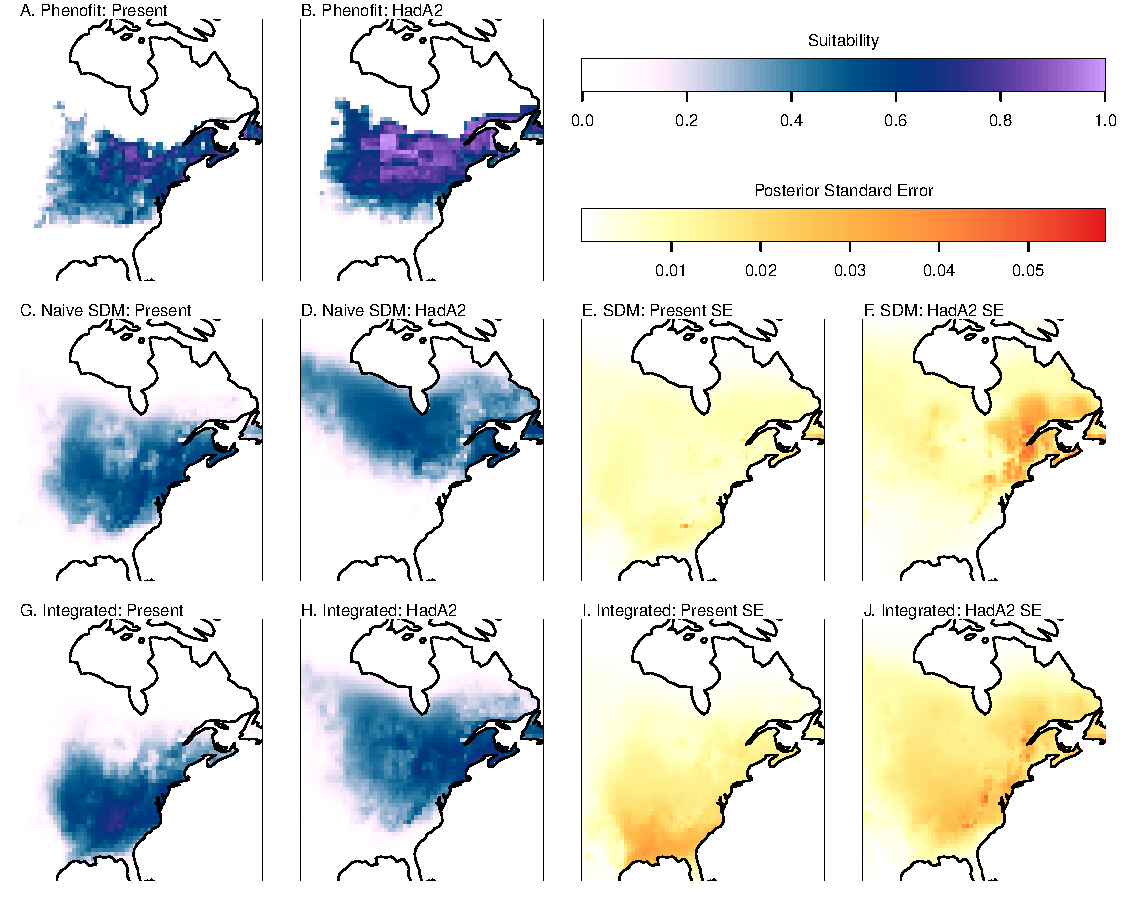
\includegraphics[width=6in]{ex2.pdf}
	\caption{Results of model integration for sugar maple, \emph{Acer saccharum}.
	The mechanistic sub-model Phenofit predicts present (A) and future (B) suitability using phenological information, but does not provide estimates of uncertainty.
	Predictions from a naive metal-model for the present (C) were quite similar to the sub-model, but future predictions (D) were somewhat different, and uncertainty was extreme at the predicted range margins for both present (E) and future (F).
	Applying the integration results in reduced suitability overall, possibly due to overfitting regions where the models disagree, but patterns in relative suitability largely reflected information from both models for both present (G) and future (H) climate.
	Integrated model uncertainty for both present (I) and future (J) climates is reduced near range margins but slightly increased in areas where uncertainty was low in the naive model.
	}
	\label{fig:ex2}
\end{figure}
%
% ERUGIF
%==================

For modeling the contemporary range of sugar maple, both Phenofit and the naive model perform very well relative to the integrated model, espeicially when capturing the range margin (Fig \ref{fig:ex2}A, C, G).
Conventional SDMs are quite good at producing empirical models of species distributions under present climatic regimes, and the naive model here could be further improved with the addition of more parameters or the inclusion of ensemble forecasting (See SI for model-fitting details).
However, Phenofit and the naive model differ substantially in their predictions of the future distribution of the species.
The integrated model presents a compromise between the two predictions. 
The core range of the species under the integrated model generally reflects the regions of highest overlap between Phenofit and the naive model.
Regions surrounding the core range generally show low suitabilities, but higher than those under either sub-model, demonstrating reduced certainty about where the species will be absent in the future.


